%!TEX root = ../main.tex
%%%%%%%%%%%%%%%%%%%%%%%%%%%%%%%%%%
% Links:
%
% Difficulty:
% Companies: 
%%%%%%%%%%%%%%%%%%%%%%%%%%%%%%%%%%

\chapter{Clone a linked list with random pointer}
\label{ch:clone_list_random_pointer}
\section*{Introduction}
This section discusses a very cool and interesting problem on linked list. The linked list we are dealing with here is a singly linked one, with an additional pointer that \textbf{might} point to another node in the list. The C++ definition of said list is given in Listing \ref{list:clone_list_random_pointer:list_definition}. Please note the additional field \lstinline[columns=fixed]{random} which differentiates it from other linked list definitions seen in other chapters (See Capter \ref{ch:delete_duplicates_list} and Listing \ref{list:delete_duplicates_list:linked_list}).

\begin{lstlisting}[language=c++, caption={Definition of a linked list with a random pointer.},label=list:delete_duplicates_list:linked_list]

template <class T> 
class Node
{
    public:
  T val;
  Node *next;
  Node *random;

  Node(const T &_val)
  {
    val    = _val;
    next   = nullptr;
    random = nullptr;
  }
};
\end{lstlisting}

\section{Problem statement}
\begin{exercise}
Given a linked list of the type defined in Listing \ref{list:clone_list_random_pointer:list_definition} return a deep-copy of it.
\end{exercise}

In this chapter we will be representing graphically a list using a list of pairs of integers. Each pair $(v,r)$ represent a node of the list where:
\begin{itemize}
	\item[-] $v$ is the payload of the node
	\item[-] $r$ is the index of the node that the random pointer points to. $-1$ represents \lstinline[columns=fixed]{nullptr}.
\end{itemize} 
For instance the list: $[(7,-1),(13,0),(11,4),(10,2),(1,0)]$ represent the list shown in Figure \ref{fig:clone_list_random_pointer:list1}.

\begin{figure}
	\label{fig:clone_list_random_pointer:list1}
	\centering
	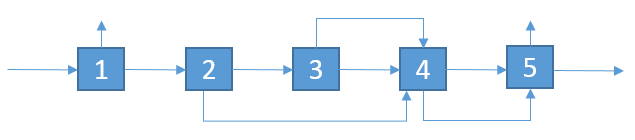
\includegraphics[scale=0.6]{sources/clone_list_random_pointer/images/random_list_1}
	\caption{Linked list wit random pointer.}
\end{figure}


\section{Clarification Questions}
The problem is clearly aimed at testing the list manipulation and it is not really about algorithm design. So question related to the size of the input do not help much. Instead it is better to ask question related to the structure of the list itself to see if there is any pattern in the lists we can take advantage of.
\begin{QandA}
	\item Is it guaranteed that at least one not-null random pointer exists?
	\begin{answered}
		\textit{No, all random pointer might be null.}
	\end{answered}
	\item Can a random pointer point to itself?
	\begin{answered}
		\textit{Yes, you can have a node pointing to itself.}
	\end{answered}
	
\end{QandA}

\section{Discussion}
\label{clone_list_random_pointer:sec:discussion}
The two solutions presented in this chapter are fundamentally different and comes with asymptotic performances differences in memory.
The solution presented in Section \ref{clone_list_random_pointer:sec:bruteforce} uses additional memory (linear amount) while the second one works in constant time but it is harder to digest and to come up with in the first place.

\subsection{Linear memory solution}
\label{clone_list_random_pointer:sec:bruteforce}
The solution presented in this section can be split into a number of distinct steps:
\begin{enumerate}
	\item Create a copy of the list with all the  next and random pointers set to \lstinline[columns=fixed]{nullptr}. Save all the pointers in an \lstinline[columns=fixed]{std::vector<Node<T>*> ptrs;}.
	\item For each node in the input list, while traversing it, save in a \lstinline[columns=fixed]{map<Node<T>*, int> P} the index of that node in the list. We want to remember for each pointer the index where it appears in the original input list. 
	\item Fix the next pointers of all nodes s.t. \lstinline[columns=fixed]{ptrs[i]->next} points to  \lstinline[columns=fixed]{ptrs[i+1]}. At this point we have a new singly linked list with broken random pointers. Basically an half cloned list.
	\item At this point we can traverse the original list once again, and if the current node $c$ has a not-null random pointer $c->p$ we can query $P$ to see which index \lstinline[columns=fixed]{P[c->p]} has in the input. We know then that we need connect also the corresponding element of $c$ in the copy with the node of index \lstinline[columns=fixed]{P[c->p]} in the copy.
\end{enumerate}

The idea above can be implemented as shown in the Listing \ref{list:clone_list_random_pointer_1}


\lstinputlisting[language=c++, caption={Linear Memory solution to the problem of copying a linked list with random pointers.},label=list:clone_list_random_pointer_1]{sources/clone_list_random_pointer/clone_list_random_pointer_solution1.cpp}

This approach has a complexity of $O(n)$ for both time and space. The time complexity is already optimal as we cannot do better than linear time, considering that to do a copy we need to look at all the nodes at least once. The space complexity can be improved though, and as we will see in Section \ref{clone_list_random_pointer:sec:interleaved_lists} it can be brought down to constant.

\subsection{Constant memory solution}
\label{clone_list_random_pointer:sec:interleaved_lists}
\subsubsection{Copy interleaved with the original list}
The idea behind the solution presented in this section is to construct the copy such that its nodes are interleaved with the ones from the original list. For instance given the input list\footnote{Remember that $(x,-1)$ is a node containing the value $x$ and with random pointer set to \lstinline[columns=fixed]{nullptr}}: $A = [(7,-1),(13,0),(11,4),(10,2),(1,0)]$ we want to have an interleaved list that look like the following: $A' = [(7,-1),(7,-1),(13,0),(13,-1),(11,4),,(11,-1),(10,2),(10,-1),(1,0),(1,0)]$ (see Figure \ref{fig:clone_list_random_pointer:interleaved}) where every node at even indexes is a copy of its predecessor with a random pointer set to \lstinline[columns=fixed]{nullptr}.  See function \lstinline[columns=fixed]{fix_random_pointers} in Listing \ref{list:clone_list_random_pointer_2}.


\begin{figure}
	\label{fig:clone_list_random_pointer:interleaved}
	\centering
	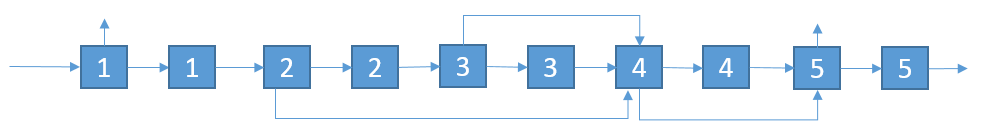
\includegraphics[scale=0.5]{sources/clone_list_random_pointer/images/random_list_2}
	\caption{Intermediate interleaved list.}
\end{figure}


In more abstract terms given:
\begin{itemize}
	\item[-] the input list  $A= a_0 \rightarrow a_1 \rightarrow \ldots \rightarrow a{n-1}$
	\item[-] a copy of A  $B = b_0 \rightarrow b_1 \rightarrow \ldots \rightarrow b{n-1}$ 
\end{itemize}

\subsubsection{Fix the random pointers in the interleaved list}
Then we want to get a list $I$ of size $2n$: $I=a_0 \rightarrow b_0 \rightarrow a_1 \rightarrow b_1 \rightarrow a_2 \rightarrow b_2 \rightarrow \ldots \rightarrow a_{n-1} \rightarrow b_{n-1}$. Having the two lists arranged this ways is quite useful because we can still visit the original lists and at the same time operate on its mirror one by simply modifying the nodes at odd indexes. An interleaved list has a even number of nodes. All the ones at even positions $(0,2,\ldots)$ belong to the original lists while all the nodes with odd indexes $(1,3,\ldots)$ to the copy. Given a node $n_{2k}=(x,r)$ at an even index $2k$, we can fix the random pointer for the clone of this node $n_{2k+1}=(x,-1)$ at index $2k+1$ by simply fixing its random pointer to the value pointed by $n_{2k}$\lstinline[columns=fixed]{->random->next}. See Figure \ref{fig:clone_list_random_pointer:interleaved_fixed} where the red lines represent the mirrored for the random pointers in the original list and function \lstinline[columns=fixed]{split_fix_random_pointers} in Listing \ref{list:clone_list_random_pointer_2}.

\begin{figure}
	\label{fig:clone_list_random_pointer:interleaved_fixed}
	\centering
	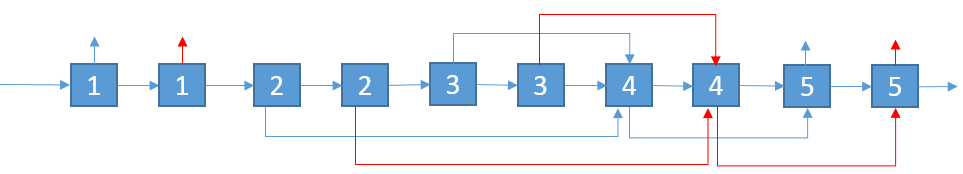
\includegraphics[scale=0.5]{sources/clone_list_random_pointer/images/random_list_3}
	\caption{Interleaved list with fixed random pointers.}
\end{figure}

\subsubsection{Extract the cloned list}
Once we reach this point we have basically two copies of the original list (with random pointers fixed) interleaved with each other. All is it necessary at this point is pull out the cloned list from the interleaved one. This is easily achievable as all we need to do is to remove all the odd nodes, and in the process connect all together (see function \lstinline[columns=fixed]{split_list} in Listing \ref{list:clone_list_random_pointer_2}).


\lstinputlisting[language=c++, caption={Constant memory solution to the problem of copying a linked list with random pointers using an interleaved list.},label=list:clone_list_random_pointer_2]{sources/clone_list_random_pointer/clone_list_random_pointer_solution2.cpp}